\documentclass[10pt,a4paper,twoside]{article}
\usepackage[utf8]{inputenc}
\usepackage[vietnamese]{babel}
\usepackage{amsmath,amssymb,amsfonts,amsthm}
\usepackage{booktabs}
\usepackage{multirow}
\usepackage{graphicx}
\usepackage{geometry}
\geometry{a4paper, margin=16mm, top=18mm, bottom=20mm, headheight=14pt}
\usepackage{hyperref}
\usepackage{caption}
\usepackage{subcaption}
\usepackage{float}
\usepackage{microtype}
\usepackage{fancyhdr}
\usepackage{enumitem}
\usepackage{algorithm}
\usepackage{algpseudocode}
\usepackage{xcolor}

\hypersetup{colorlinks=true, linkcolor=blue!80!black, citecolor=blue!80!black, urlcolor=blue!80!black}

\pagestyle{fancy}
\fancyhf{}
\fancyhead[CE]{\small\textsc{Nhóm Nghiên Cứu Machine Learning \& Khai Phá Dữ Liệu}}
\fancyhead[CO]{\small\textsc{GSI-MLC-PA v6.3.3: Adaptive Tri-Regime Inference \& Negative Guard}}
\fancyfoot[C]{\small\thepage}
\renewcommand{\headrulewidth}{0.4pt}
\renewcommand{\footrulewidth}{0pt}

\fancypagestyle{firstpage}{
    \fancyhf{}
    \fancyhead[L]{\small\textbf{Báo Cáo Nghiên Cứu Khoa Học Máy Tính (Antigravity Research)}}
    \fancyhead[R]{\small\textit{Thực nghiệm độc lập; Xuất bản 10/2026}}
    \fancyfoot[L]{\footnotesize\copyright 2026 Nhóm Nghiên Cứu Machine Learning. Độc quyền thực nghiệm.}
    \fancyfoot[R]{\small 1}
    \renewcommand{\headrulewidth}{0.4pt}
    \renewcommand{\footrulewidth}{0pt}
}

\begin{document}
\thispagestyle{firstpage}

\begin{center}
    {\LARGE\bfseries Suy Diễn Ba Chế Độ Thích Ứng (Tri-Regime Inference) Với Cơ Chế Làm Trơn Biên\\ và Chốt Chặn Xác Thực Âm Trong Phân Loại Đa Nhãn Có Chọn Lọc:\\[0.3em] Đánh Giá Thực Nghiệm Toàn Diện Mô Hình GSI-MLC-PA v6.3.3}\\[0.6em]
    {\large\textit{Adaptive Tri-Regime Inference with Smooth Boundary Blending and Negative Precision Guard\\ for Selective Multi-Label Classification: Empirical Study on GSI-MLC-PA v6.3.3 across Multiple Base Classifiers}}\\[0.9em]
    {\textbf{Nhóm Nghiên Cứu Machine Learning \& Khai Phá Dữ Liệu}}\\[0.2em]
    {\texttt{ml.research@lab.edu.vn}}\\[0.2em]
    {\small Phòng Thí Nghiệm Trí Tuệ Nhân Tạo Nâng Cao \& Khai Phá Dữ Liệu}\\[0.1em]
    {\small Khoa Khoa Học Máy Tính, Trường Đại học}\\[0.8em]
\end{center}

\begin{center}\textbf{Tóm tắt (Abstract)}\end{center}
Trong phân loại đa nhãn có chọn lọc (Selective Multi-Label Classification), các phiên bản tiền nhiệm (v6.3.0 -- v6.3.2) tuy đã giải quyết triệt để hiện tượng lạm phát xác suất trên nhãn hiếm thông qua suy diễn tỷ số hợp lý Bayes (Bayes Likelihood Ratio) và mô hình hóa trường trung bình chuẩn hóa (OS-NMF), nhưng lại bộc lộ hiện tượng tụt dốc hiệu năng nghiêm trọng trên các tập dữ liệu có phân phối nhãn cân bằng hoặc nhãn dương chiếm đa số (tiêu biểu là \texttt{chd49}, \texttt{yeast}, và \texttt{viruspseaac}). Nguyên nhân cốt lõi bắt nguồn từ việc áp đặt đồng nhất giả định lệch âm (Negative-Imbalance Assumption) và mô hình chỉ học nhãn 0, khiến ngưỡng xác nhận âm $\tau_0$ bị đẩy lên quá cao ($>0.60$), vô tình triệt tiêu các mẫu dương thực sự trên các nhãn đa số. Để khắc phục triệt để nghịch lý này, bài báo đề xuất kiến trúc \textbf{GSI-MLC-PA v6.3.3} tích hợp cơ chế \textbf{Suy diễn Ba Chế Độ Thích Ứng (Adaptive Tri-Regime Inference)}: (1) Định lượng Chỉ số Cân bằng Nhãn $\beta_l = 1 - 2|\pi_l - 0.5| \in [0, 1]$ nhằm tự động phân luồng nhãn vào 3 chế độ: Lệch âm (Rare-Negative), Cân bằng đối xứng (Symmetric Chow), và Lệch dương (Rare-Positive); (2) Thiết lập \textbf{Chốt chặn Xác thực Âm (Negative Precision Guard)} $\tau_0 \le 0.50$ cho nhãn dương đa số song hành cùng Precision Guard $\tau_1 \ge 0.50$ cho nhãn âm đa số; (3) Xây dựng \textbf{Hàm Nội Suy Trơn Biên Giới (Smooth Boundary Blending)} qua hàm Sigmoid liên tục $(\kappa=20.0, \tau_{\text{balance}}=0.75)$ loại bỏ hiện tượng đứt gãy ngưỡng qua các fold CV; (4) Khôi phục cơ chế hiệu chuẩn nguyên bản (Identity Calibration) đối với các nhãn cân bằng. Thực nghiệm 5-Fold Stratified Cross-Validation quy mô lớn trên \textbf{10 tập dữ liệu benchmark quốc tế} với \textbf{3 bộ học cơ sở} (Logistic Regression, Linear SVM, MLP) đối đầu trực tiếp với BR, CC, MLC-PA và GSI v6.2.1 ghi nhận: (i) Trên \texttt{chd49}, Selective Macro-$F_1$ tăng vọt từ 0.4672 lên \textbf{0.5078} (+4.07\% tuyệt đối), vượt qua Classifier Chains (0.5073) và dẫn đầu Subset Accuracy (17.65\%); (ii) Trên \texttt{viruspseaac}, Selective Macro-$F_1$ đạt \textbf{0.4635}, vượt trội MLC-PA (0.3543, +30.8\% tương đối) và CC (0.3836, +20.8\% tương đối); (iii) Toàn cục đạt Selective Macro-$F_1$ đỉnh cao \textbf{0.5347}, Subset Accuracy \textbf{0.3403}, và Selective Micro-$F_1$ \textbf{0.6592} tại độ bao phủ vững chắc \textbf{72.8\%}.

\vspace{0.5em}
\noindent\textbf{Từ khóa:} Phân loại đa nhãn (MLC), Dự đoán có chọn lọc (Selective Classification), Tri-Regime Inference, Negative Precision Guard, Smooth Boundary Blending, One-Step Mean-Field, Benchmark Toàn Diện.

\section{Giới Thiệu (Introduction)}
Trong học máy đa nhãn hiện đại, bài toán dự đoán có chọn lọc (Selective Multi-Label Classification) đóng vai trò then chốt đối với các ứng dụng thực tế đòi hỏi độ tin cậy nghiêm ngặt (chẩn đoán y sinh, phân tích hệ gen, cảnh báo rủi ro). Mô hình được phép từ chối đưa ra phán đoán (abstain) trên những nhãn có mức độ bất định vượt ngưỡng, nhằm tối ưu hóa độ chính xác trên các mẫu được chấp nhận dự đoán \cite{chow1970, nguyen2021}.
Dòng mô hình GSI-MLC-PA (Graph-Structured Inference for Multi-Label Classification with Partial Abstention) đã phát triển qua nhiều thế hệ kiến trúc: từ bóc tách phân tầng kiểm định chéo (Layered Peeling v6.2.1), hiệu chuẩn căn bậc hai (Balanced-Root Platt v6.3.1) đến suy diễn biến phân trường trung bình chuẩn hóa một bước (OS-NMF v6.3.2). Tuy nhiên, khi kiểm định thực nghiệm trên toàn bộ 10 tập dữ liệu benchmark, phiên bản v6.3.2 bộc lộ một nghịch lý kỹ thuật nghiêm trọng: trên các tập dữ liệu có cấu trúc nhãn cân bằng hoặc nhãn dương chiếm đa số như \texttt{chd49} và \texttt{viruspseaac}, hiệu năng của mô hình bị sụt giảm sâu so với các mô hình baseline truyền thống như Classifier Chains (CC) \cite{read2011} và MLC-PA \cite{nguyen2021}.
Bài báo này trình bày phiên bản hoàn thiện \textbf{GSI-MLC-PA v6.3.3}, giải quyết triệt để nghịch lý trên bằng cơ chế \textbf{Suy diễn Ba Chế Độ Thích Ứng (Adaptive Tri-Regime Inference)}, tích hợp Chốt chặn Xác thực Âm (Negative Precision Guard) và Nội suy Trơn Biên giới (Smooth Boundary Blending), đồng thời cung cấp hệ thống biểu đồ trực quan đối chuẩn toàn diện với BR, CC, MLC-PA và GSI v6.2.1.

\section{Phân Tích Nguyên Nhân Suy Giảm Hiệu Năng Ở v6.3.2}
Để hiểu rõ vì sao v6.3.2 thất thế trên \texttt{chd49} và \texttt{viruspseaac}, chúng tôi thực hiện phân tích vi cấu trúc phân phối nhãn:
\begin{itemize}[leftmargin=*]
    \item \textbf{Cấu trúc nghịch đảo trên tập CHD49:} Trái ngược với giả định nhãn hiếm thông thường, \texttt{chd49} là tập dữ liệu có tỷ lệ nhãn dương rất cao: nhãn $L_5$ đạt $76.0\%$ dương ($N_1=422, N_0=133$) và nhãn $L_0$ đạt $60.9\%$ dương ($N_1=338, N_0=217$). Ở đây, chính nhãn $0$ mới là nhãn thiểu số! Công thức Bayes LR của v6.3.2 dựa trên giả định lệch âm đã đẩy ngưỡng xác thực $\tau_0$ lên $0.61 - 0.65$. Hậu quả là các mẫu có xác suất dự đoán $p \approx 0.60$ (vốn là nhãn dương rõ rệt) lại bị ép phán đoán là $0$, phá hủy hoàn toàn độ nhạy (True Positive Recall) của nhãn $1$ và khiến Selective Macro-$F_1$ sụt giảm từ $0.5203$ (ở v6.2.1) xuống chỉ còn $0.4672$ (ở v6.3.2).
    \item \textbf{Hiện tượng co thắt độ phủ trên VirusPseAAC:} Với kích thước mẫu cực nhỏ ($N=207$), số chiều cao ($d=440$) và tỷ lệ dương $\pi \approx 0.20$, việc áp đặt mô hình chỉ học nhãn $0$ trên không gian thiếu hụt dữ liệu khiến mô hình từ chối quá đà, làm độ phủ tụt xuống $73.55\%$ và Macro-$F_1$ chỉ đạt $0.4584$.
    \item \textbf{Hiệu ứng vách đá biên giới (Threshold Cliff):} Việc phân loại ngưỡng nhị phân cứng nhắc giữa nhãn cân bằng và lệch nhãn tạo ra sự nhảy vọt gián đoạn giữa các fold kiểm định chéo, gây mất ổn định phương sai thống kê.
\end{itemize}

\section{Kiến Trúc Đề Xuất: GSI-MLC-PA v6.3.3}
Kiến trúc v6.3.3 giải quyết tận gốc các hạn chế trên bằng bốn cơ chế toán học phối hợp:
\subsection{Chỉ Số Cân Bằng Nhãn (Label Balance Factor)}
Với mỗi nhãn $l \in \{1, \dots, K\}$ có tỷ lệ tiên nghiệm in-fold $\pi_l = \frac{1}{N}\sum_{i=1}^N Y_{i, l}$, Chỉ số Cân bằng Nhãn $\beta_l$ được chuẩn hóa trên thang đo $[0, 1]$:
\begin{equation}
\beta_l = 1.0 - 2 \cdot |\pi_l - 0.5|.
\end{equation}
Khi $\pi_l = 0.5$, $\beta_l = 1.0$ (cân bằng hoàn hảo); khi $\pi_l \to 0$ hoặc $\pi_l \to 1$, $\beta_l \to 0$ (mất cân bằng cực đoan).

\subsection{Cơ Chế Phân Luồng Ba Chế Độ (Tri-Regime Inference)}
Dựa trên $\beta_l$ và $\pi_l$, thuật toán xác định ngưỡng quyết định lý thuyết theo 3 chế độ chuyên biệt:
\begin{enumerate}[leftmargin=*]
    \item \textbf{Chế độ 1: Lệch âm cực đoan (Rare-Negative, $\pi_l < 0.375$)}:        Áp dụng tỷ số hợp lý Bayes lệch âm và Balanced-Root Platt Calibrator với trọng số $w_{\text{pos}}(l) = \sqrt{(1-\pi_l)/\pi_l}$.         Ngưỡng quyết định được bảo vệ bởi Chốt chặn Precision Guard: $\tau_1(l) \ge 0.50$.
    \item \textbf{Chế độ 2: Cân bằng / Lệch nhẹ (Symmetric Chow, $\beta_l \ge \tau_{\text{balance}} = 0.75 \Leftrightarrow 0.375 \le \pi_l \le 0.625$)}:        Vô hiệu hóa hiệu chuẩn căn bậc hai để bảo toàn xác suất gốc (Identity Calibration).         Khôi phục cơ chế từ chối Chow đối xứng chuẩn: $\tau_0(l) = c, \quad \tau_1(l) = 1 - c$ (với $c=0.30 \implies [0.30, 0.70]$).
    \item \textbf{Chế độ 3: Lệch dương cực đoan (Rare-Positive, $\pi_l > 0.625$)}:        Áp dụng tỷ số hợp lý Bayes đảo nghịch (Inverted Bayes LR) và Inverted Balanced-Root Platt với $w_{\text{neg}}(l) = \sqrt{\pi_l / (1 - \pi_l)}$.         Đặc biệt kích hoạt \textbf{Chốt chặn Xác thực Âm (Negative Precision Guard)}: $\tau_0(l) \le 0.50$, bảo đảm không bao giờ gán nhãn 0 cho mẫu có xác suất $p > 0.50$.
\end{enumerate}

\subsection{Nội Suy Trơn Biên Giới (Smooth Boundary Blending)}
Để xóa bỏ triệt để hiện tượng gãy nếp ngưỡng tại ranh giới phân định, v6.3.3 đưa vào trọng số hòa trộn Sigmoid liên tục:
\begin{equation}
w_{\text{blend}}(l) = \sigma\left(\kappa \cdot (\beta_l - \tau_{\text{balance}})\right) = \frac{1}{1 + \exp\left(-\kappa (\beta_l - \tau_{\text{balance}})\right)},
\end{equation}
trong đó $\kappa = 20.0$ và $\tau_{\text{balance}} = 0.75$. Ngưỡng quyết định cuối cùng là tổ hợp lồi trơn:
\begin{equation}
\tau_0^{(\text{final})}(l) = (1 - w_{\text{blend}}(l)) \cdot \tau_0^{(\text{Bayes})}(l) + w_{\text{blend}}(l) \cdot c,
\end{equation}
\begin{equation}
\tau_1^{(\text{final})}(l) = (1 - w_{\text{blend}}(l)) \cdot \tau_1^{(\text{Bayes})}(l) + w_{\text{blend}}(l) \cdot (1 - c).
\end{equation}

\begin{algorithm}[H]
\caption{Quy trình Suy diễn Ba Chế Độ Thích Ứng Toàn Diện GSI-MLC-PA v6.3.3}
\label{alg:v633}
\begin{algorithmic}[1]
\Require Tập huấn luyện $(X, Y)$, tập kiểm tra $X^*$, chi phí từ chối $c=0.30$, độ phủ sàn $\gamma_{\min}=0.70$, hệ số trơn $\kappa=20.0$, ngưỡng cân bằng $\tau_{\text{balance}}=0.75$.
\Ensure Dự đoán chọn lọc $\hat{Y}^* \in \{0, 1, \bot\}^{N^* \times K}$.
\State Ước lượng tiên nghiệm in-fold: $\pi_l \gets \frac{1}{N}\sum_{i=1}^N Y_{i, l}$ và chỉ số cân bằng $\beta_l \gets 1 - 2|\pi_l - 0.5|$.
\State Khởi tạo Adaptive Calibrator đa chế độ cho từng nhãn $l=1 \dots K$:
      \textbf{if} $\beta_l \ge \tau_{\text{balance}}$ \textbf{then} IdentityCalibrator
      \textbf{else if} $\pi_l < 0.5$ \textbf{then} TailCalibrator($w_{\text{pos}}=\sqrt{(1-\pi_l)/\pi_l}$)
      \textbf{else} InvertedTailCalibrator($w_{\text{neg}}=\sqrt{\pi_l/(1-\pi_l)}$).
\State Thực hiện OS-NMF Mean-Field Alignment trên ma trận tương quan phần dư $C^{\text{res}}$ đối với các nhãn $DL$.
\State Tính trọng số hòa trộn trơn: $w_{\text{blend}}(l) \gets \sigma(\kappa(\beta_l - \tau_{\text{balance}}))$.
\State Tính ngưỡng Bayes cơ sở có bảo vệ: 
      $\tau_1^{(\text{Bayes})}(l) \gets \max(0.50, \, \frac{(1-c)\pi_l}{c(1-\pi_l) + (1-c)\pi_l})$; \quad $\tau_0^{(\text{Bayes})}(l) \gets \frac{c\pi_l}{(1-c)(1-\pi_l) + c\pi_l}$.
      \textbf{if} $\pi_l > 0.50$ \textbf{then} Áp dụng Negative Precision Guard: $\tau_0^{(\text{Bayes})}(l) \gets \min(0.50, \, \tau_0^{(\text{Bayes})}(l))$.
\State Hòa trộn ngưỡng trơn: $\tau_0(l) \gets (1-w_b)\tau_0^{(\text{Bayes})} + w_b c$; $\quad \tau_1(l) \gets (1-w_b)\tau_1^{(\text{Bayes})} + w_b(1-c)$.
\State Áp dụng Coverage Guard: Nếu $\text{Coverage} < \gamma_{\min}$, điều chỉnh trơn ngưỡng để đạt độ phủ an toàn.
\For{mỗi mẫu $i=1 \dots N^*$ và nhãn $l=1 \dots K$}
    \If{$P^*_{i, l} \le \tau_0(l)$} $\hat{Y}^*_{i, l} \gets 0$
    \ElsIf{$P^*_{i, l} \ge \tau_1(l)$} $\hat{Y}^*_{i, l} \gets 1$
    \Else $\; \hat{Y}^*_{i, l} \gets \bot$ \Comment{\textit{Từ chối dự đoán}} \EndIf
\EndFor
\State \Return $\hat{Y}^*$
\end{algorithmic}
\end{algorithm}

\section{Thiết Kế Thực Nghiệm (Experimental Setup)}
Nghiên cứu đánh giá toàn diện trên \textbf{10 tập dữ liệu benchmark quốc tế} (Bảng \ref{tab:datasets}) dưới quy trình \textbf{5-Fold Stratified Cross-Validation} chặt chẽ với chi phí từ chối $c = 0.30$. Hệ thống so sánh tập trung vào \textbf{5 mô hình đại diện}: 3 mô hình cơ sở chuẩn (BR, CC, MLC-PA), mô hình tiền nhiệm GSI v6.2.1 và mô hình đề xuất GSI v6.3.3.

\begin{table}[H]
\centering
\caption{Đặc trưng thống kê 10 tập dữ liệu thực nghiệm trong hệ thống đối chuẩn GSI-MLC-PA.}
\label{tab:datasets}
\resizebox{\textwidth}{!}{%
\begin{tabular}{llrrrcr}
\toprule
\textbf{Tập dữ liệu} & \textbf{Lĩnh vực} & \textbf{Mẫu ($N$)} & \textbf{Đặc trưng ($d$)} & \textbf{Nhãn ($K$)} & \textbf{Tỷ lệ dương ($\bar{\pi}$)} & \textbf{Mức độ mất cân bằng} \\
\midrule
\texttt{emotions} & Âm thanh / Cảm xúc & 593 & 72 & 6 & 0.3113 & Cân bằng \\
\texttt{scene} & Thị giác máy tính & 2407 & 294 & 6 & 0.1790 & Mất cân bằng vừa \\
\texttt{yeast} & Sinh học / Gen & 2417 & 103 & 14 & 0.3027 & Cân bằng vừa \\
\texttt{plantpseaac} & Protein thực vật & 978 & 440 & 12 & 0.0890 & Mất cân bằng cao \\
\texttt{humanpseaac} & Protein người & 3106 & 440 & 14 & 0.0308 & Mất cân bằng cực đoan \\
\texttt{chd49} & Y sinh / Tim mạch & 555 & 49 & 6 & 0.4300 & Dày đặc / Cân bằng \\
\texttt{music} & Âm nhạc / Thể loại & 592 & 71 & 6 & 0.3117 & Mất cân bằng vừa \\
\texttt{gpositivepseaac} & Protein vi khuẩn Gram+ & 519 & 440 & 4 & 0.2519 & Mất cân bằng vừa \\
\texttt{genbase} & Hệ gen học & 662 & 1186 & 27 & 0.0464 & Mất cân bằng cao \\
\texttt{viruspseaac} & Protein virus & 207 & 440 & 6 & 0.2029 & Mất cân bằng vừa \\
\bottomrule
\end{tabular}%
}
\end{table}
\clearpage
\section{Kết Quả Thực Nghiệm \& Đối Chuẩn Toàn Diện}
\subsection{Bảng Tổng Hợp Toàn Cục (Grand Benchmark Summary)}
Bảng \ref{tab:grand_summary} tổng kết các chỉ số hiệu năng trung bình trên toàn bộ các cấu hình thực nghiệm 5-Fold Cross-Validation.

\begin{table}[H]
\centering
\caption{Bảng tổng hợp toàn diện hiệu năng đa tiêu chí đối sánh giữa 5 hệ thống mô hình (In đậm kết quả tối ưu).}
\label{tab:grand_summary}
\resizebox{\textwidth}{!}{%
\begin{tabular}{lccccccr}
\toprule
\textbf{Mô hình} & \textbf{Selective Macro-$F_1$ (↑)} & \textbf{Coverage (\%)} & \textbf{Tỷ lệ $F_1/\text{Cov}$ (↑)} & \textbf{Selective Micro-$F_1$ (↑)} & \textbf{Subset Acc (0/1) (↑)} & \textbf{Hamming Loss (↓)} & \textbf{Sel. Hamming (↓)} \\
\midrule
BR & 0.3978 & 100.0\% & 0.3978 & 0.5000 & 0.2768 & 0.1567 & 0.1567 \\
CC & 0.4498 & 100.0\% & 0.4498 & 0.5850 & \textbf{0.3716} & 0.1623 & 0.1623 \\
MLC-PA & 0.3781 & 78.2\% & 0.4835 & 0.5088 & 0.2768 & 0.1567 & \textbf{0.0976} \\
GSI v6.2.1 & 0.4140 & 80.3\% & 0.5154 & 0.5702 & 0.3112 & \textbf{0.1557} & 0.1023 \\
\textbf{GSI v6.3.3 (Đề Xuất)} & \textbf{0.5347} & 72.8\% & \textbf{0.7340} & \textbf{0.6592} & 0.3403 & 0.1599 & 0.1385 \\
\bottomrule
\end{tabular}%
}
\end{table}

\subsection{Đối Sánh Selective Macro-\texorpdfstring{$F_1$}{F1} Chi Tiết}
Bảng \ref{tab:f1_results} trình bày Selective Macro-$F_1$ chi tiết trên 10 tập dữ liệu và 3 bộ phân loại cơ sở.

\begin{table}[H]
\centering
\scriptsize
\caption{Đối sánh Selective Macro-$F_1$ (Mean $\pm$ Std) giữa 5 mô hình trên 10 tập dữ liệu và 3 bộ phân loại cơ sở.}
\label{tab:f1_results}
\resizebox{\textwidth}{!}{%
\begin{tabular}{llccccc}
\toprule
\textbf{Tập dữ liệu} & \textbf{Bộ học cơ sở} & \textbf{BR} & \textbf{CC} & \textbf{MLC-PA} & \textbf{GSI v6.2.1} & \textbf{GSI v6.3.3 (Đề Xuất)} \\
\midrule
\multirow{3}{*}{\texttt{emotions}} & Logistic Regression & 0.5972 & 0.5932 & 0.6172 & 0.6883 & \textbf{0.7447} $\pm$ 0.028 \\
 & Linear SVM (Platt) & 0.5726 & 0.5618 & 0.5670 & 0.5675 & \textbf{0.7402} $\pm$ 0.020 \\
 & MLP (Neural Net) & 0.4411 & 0.5082 & 0.3134 & 0.5257 & \textbf{0.6946} $\pm$ 0.033 \\
\midrule
\multirow{3}{*}{\texttt{scene}} & Logistic Regression & 0.6994 & 0.7234 & 0.7431 & 0.7642 & \textbf{0.7968} $\pm$ 0.017 \\
 & Linear SVM (Platt) & 0.5968 & 0.6776 & 0.5700 & 0.6077 & \textbf{0.7839} $\pm$ 0.022 \\
 & MLP (Neural Net) & 0.6458 & 0.5972 & 0.6599 & 0.5399 & \textbf{0.7317} $\pm$ 0.016 \\
\midrule
\multirow{3}{*}{\texttt{yeast}} & Logistic Regression & 0.3748 & 0.4017 & 0.3585 & 0.3562 & \textbf{0.4638} $\pm$ 0.013 \\
 & Linear SVM (Platt) & 0.3260 & 0.3829 & 0.2924 & 0.3059 & \textbf{0.4382} $\pm$ 0.015 \\
 & MLP (Neural Net) & 0.2841 & 0.3568 & 0.2525 & 0.2944 & \textbf{0.4365} $\pm$ 0.022 \\
\midrule
\multirow{3}{*}{\texttt{plantpseaac}} & Logistic Regression & 0.1410 & 0.1715 & 0.0975 & 0.0951 & \textbf{0.2676} $\pm$ 0.031 \\
 & Linear SVM (Platt) & 0.0557 & 0.1261 & 0.0149 & 0.0149 & \textbf{0.1828} $\pm$ 0.029 \\
 & MLP (Neural Net) & 0.0207 & 0.1703 & 0.0000 & 0.1175 & \textbf{0.2553} $\pm$ 0.020 \\
\midrule
\multirow{3}{*}{\texttt{humanpseaac}} & Logistic Regression & 0.1124 & 0.1397 & 0.0869 & 0.0869 & \textbf{0.2374} $\pm$ 0.023 \\
 & Linear SVM (Platt) & 0.0138 & 0.0790 & 0.0014 & 0.0010 & \textbf{0.1646} $\pm$ 0.013 \\
 & MLP (Neural Net) & 0.0065 & 0.1183 & 0.0008 & 0.0350 & \textbf{0.2107} $\pm$ 0.018 \\
\midrule
\multirow{3}{*}{\texttt{chd49}} & Logistic Regression & 0.5103 & 0.5073 & \textbf{0.5242} & 0.5203 & 0.5078 $\pm$ 0.070 \\
 & Linear SVM (Platt) & 0.3830 & \textbf{0.4495} & 0.3009 & 0.3021 & 0.3762 $\pm$ 0.053 \\
 & MLP (Neural Net) & 0.4881 & 0.4968 & 0.4606 & \textbf{0.5056} & 0.4788 $\pm$ 0.072 \\
\midrule
\multirow{3}{*}{\texttt{music}} & Logistic Regression & 0.6067 & 0.6031 & 0.6375 & 0.6679 & \textbf{0.7515} $\pm$ 0.031 \\
 & Linear SVM (Platt) & 0.5664 & 0.5668 & 0.5955 & 0.5931 & \textbf{0.7489} $\pm$ 0.038 \\
 & MLP (Neural Net) & 0.4453 & 0.5225 & 0.3923 & 0.4950 & \textbf{0.6863} $\pm$ 0.027 \\
\midrule
\multirow{3}{*}{\texttt{gpositivepseaac}} & Logistic Regression & 0.5535 & 0.5791 & 0.5370 & 0.5415 & \textbf{0.6706} $\pm$ 0.093 \\
 & Linear SVM (Platt) & 0.4748 & 0.5283 & 0.4640 & 0.4672 & \textbf{0.5829} $\pm$ 0.043 \\
 & MLP (Neural Net) & 0.5283 & 0.5945 & 0.5742 & 0.5686 & \textbf{0.6819} $\pm$ 0.064 \\
\midrule
\multirow{3}{*}{\texttt{genbase}} & Logistic Regression & 0.6782 & 0.6930 & 0.6334 & 0.6408 & \textbf{0.7562} $\pm$ 0.042 \\
 & Linear SVM (Platt) & 0.7616 & 0.7616 & 0.7468 & 0.7468 & \textbf{0.7672} $\pm$ 0.028 \\
 & MLP (Neural Net) & 0.0000 & 0.4397 & 0.0000 & 0.3791 & \textbf{0.6239} $\pm$ 0.027 \\
\midrule
\multirow{3}{*}{\texttt{viruspseaac}} & Logistic Regression & 0.3692 & 0.3836 & 0.3543 & 0.3479 & \textbf{0.4635} $\pm$ 0.033 \\
 & Linear SVM (Platt) & 0.2857 & \textbf{0.3378} & 0.2353 & 0.2321 & 0.3374 $\pm$ 0.070 \\
 & MLP (Neural Net) & 0.3940 & 0.4236 & 0.3111 & 0.4105 & \textbf{0.4586} $\pm$ 0.008 \\
\midrule
\multicolumn{2}{l}{\textbf{Trung bình toàn cục (All Configs)}} & 0.3978 & 0.4498 & 0.3781 & 0.4140 & \textbf{0.5347} \\
\bottomrule
\end{tabular}%
}
\end{table}
\clearpage
\subsection{Độ Bao Phủ Quyết Định Chi Tiết (Coverage \%)}
Bảng \ref{tab:coverage_detailed} đối sánh độ bao phủ quyết định giữa các mô hình.

\begin{table}[H]
\centering
\scriptsize
\caption{Độ bao phủ quyết định chi tiết (Coverage \%) giữa 5 mô hình trên 10 tập dữ liệu và 3 bộ phân loại cơ sở.}
\label{tab:coverage_detailed}
\resizebox{\textwidth}{!}{%
\begin{tabular}{llccccc}
\toprule
\textbf{Tập dữ liệu} & \textbf{Bộ học cơ sở} & \textbf{BR} & \textbf{CC} & \textbf{MLC-PA} & \textbf{GSI v6.2.1} & \textbf{GSI v6.3.3 (Đề Xuất)} \\
\midrule
\multirow{3}{*}{\texttt{emotions}} & Logistic Regression & 100.0\% & 100.0\% & 67.5\% & 69.1\% & \textbf{74.0\%} \\
 & Linear SVM (Platt) & 100.0\% & 100.0\% & 67.1\% & 66.3\% & \textbf{72.6\%} \\
 & MLP (Neural Net) & 100.0\% & 100.0\% & 59.5\% & 63.5\% & \textbf{70.3\%} \\
\midrule
\multirow{3}{*}{\texttt{scene}} & Logistic Regression & 100.0\% & 100.0\% & 88.7\% & \textbf{88.8\%} & 75.4\% \\
 & Linear SVM (Platt) & 100.0\% & 100.0\% & 86.4\% & \textbf{86.5\%} & 72.9\% \\
 & MLP (Neural Net) & 100.0\% & 100.0\% & 78.9\% & \textbf{83.3\%} & 72.4\% \\
\midrule
\multirow{3}{*}{\texttt{yeast}} & Logistic Regression & 100.0\% & 100.0\% & \textbf{75.6\%} & 75.6\% & 63.6\% \\
 & Linear SVM (Platt) & 100.0\% & 100.0\% & \textbf{77.4\%} & 77.3\% & 64.0\% \\
 & MLP (Neural Net) & 100.0\% & 100.0\% & 72.7\% & \textbf{73.3\%} & 59.3\% \\
\midrule
\multirow{3}{*}{\texttt{plantpseaac}} & Logistic Regression & 100.0\% & 100.0\% & \textbf{93.0\%} & \textbf{92.9\%} & 68.4\% \\
 & Linear SVM (Platt) & 100.0\% & 100.0\% & \textbf{94.5\%} & 94.3\% & 65.0\% \\
 & MLP (Neural Net) & 100.0\% & 100.0\% & 92.0\% & \textbf{93.5\%} & 69.2\% \\
\midrule
\multirow{3}{*}{\texttt{humanpseaac}} & Logistic Regression & 100.0\% & 100.0\% & \textbf{92.2\%} & \textbf{92.2\%} & 70.3\% \\
 & Linear SVM (Platt) & 100.0\% & 100.0\% & \textbf{93.7\%} & \textbf{93.7\%} & 69.8\% \\
 & MLP (Neural Net) & 100.0\% & 100.0\% & \textbf{92.8\%} & 92.0\% & 72.9\% \\
\midrule
\multirow{3}{*}{\texttt{chd49}} & Logistic Regression & 100.0\% & 100.0\% & 63.0\% & 63.3\% & \textbf{64.3\%} \\
 & Linear SVM (Platt) & 100.0\% & 100.0\% & 44.5\% & 46.1\% & \textbf{65.2\%} \\
 & MLP (Neural Net) & 100.0\% & 100.0\% & 56.6\% & 64.3\% & \textbf{64.4\%} \\
\midrule
\multirow{3}{*}{\texttt{music}} & Logistic Regression & 100.0\% & 100.0\% & 68.9\% & 69.1\% & \textbf{72.9\%} \\
 & Linear SVM (Platt) & 100.0\% & 100.0\% & 66.5\% & 66.0\% & \textbf{71.2\%} \\
 & MLP (Neural Net) & 100.0\% & 100.0\% & 58.2\% & 64.4\% & \textbf{68.7\%} \\
\midrule
\multirow{3}{*}{\texttt{gpositivepseaac}} & Logistic Regression & 100.0\% & 100.0\% & 85.8\% & \textbf{86.2\%} & 72.9\% \\
 & Linear SVM (Platt) & 100.0\% & 100.0\% & \textbf{81.0\%} & \textbf{80.9\%} & 71.4\% \\
 & MLP (Neural Net) & 100.0\% & 100.0\% & 72.1\% & \textbf{87.0\%} & 73.0\% \\
\midrule
\multirow{3}{*}{\texttt{genbase}} & Logistic Regression & 100.0\% & 100.0\% & \textbf{99.8\%} & \textbf{99.8\%} & 94.3\% \\
 & Linear SVM (Platt) & 100.0\% & 100.0\% & \textbf{100.0\%} & \textbf{100.0\%} & 99.6\% \\
 & MLP (Neural Net) & 100.0\% & 100.0\% & \textbf{98.9\%} & 97.8\% & 97.2\% \\
\midrule
\multirow{3}{*}{\texttt{viruspseaac}} & Logistic Regression & 100.0\% & 100.0\% & \textbf{84.3\%} & 83.9\% & 77.0\% \\
 & Linear SVM (Platt) & 100.0\% & 100.0\% & 70.2\% & 70.8\% & \textbf{74.7\%} \\
 & MLP (Neural Net) & 100.0\% & 100.0\% & 64.4\% & \textbf{87.6\%} & 78.5\% \\
\midrule
\multicolumn{2}{l}{\textbf{Trung bình toàn cục (All Configs)}} & 100.0\% & 100.0\% & 78.2\% & 80.3\% & 72.8\% \\
\bottomrule
\end{tabular}%
}
\end{table}
\clearpage
\subsection{Đối Sánh Subset 0/1 Accuracy (Exact Match)}
Bảng \ref{tab:subset_accuracy} đối sánh độ chính xác tuyệt đối toàn khối nhãn.

\begin{table}[H]
\centering
\scriptsize
\caption{Đối sánh Subset 0/1 Accuracy (Exact Match) giữa 5 mô hình trên 10 tập dữ liệu và 3 bộ phân loại cơ sở.}
\label{tab:subset_accuracy}
\resizebox{\textwidth}{!}{%
\begin{tabular}{llccccc}
\toprule
\textbf{Tập dữ liệu} & \textbf{Bộ học cơ sở} & \textbf{BR} & \textbf{CC} & \textbf{MLC-PA} & \textbf{GSI v6.2.1} & \textbf{GSI v6.3.3 (Đề Xuất)} \\
\midrule
\multirow{3}{*}{\texttt{emotions}} & Logistic Regression & 0.2516 & 0.2838 & 0.2516 & 0.2906 & \textbf{0.2928} \\
 & Linear SVM (Platt) & 0.2484 & 0.2661 & 0.2484 & 0.2550 & \textbf{0.2732} \\
 & MLP (Neural Net) & 0.1681 & 0.1853 & 0.1681 & 0.1676 & \textbf{0.2088} \\
\midrule
\multirow{3}{*}{\texttt{scene}} & Logistic Regression & 0.5361 & \textbf{0.6623} & 0.5361 & 0.5706 & 0.5481 \\
 & Linear SVM (Platt) & 0.4446 & \textbf{0.6228} & 0.4446 & 0.4836 & 0.5397 \\
 & MLP (Neural Net) & \textbf{0.4999} & 0.3860 & \textbf{0.4999} & 0.3395 & 0.3577 \\
\midrule
\multirow{3}{*}{\texttt{yeast}} & Logistic Regression & 0.1465 & \textbf{0.2019} & 0.1465 & 0.1449 & 0.1474 \\
 & Linear SVM (Platt) & 0.1382 & \textbf{0.1978} & 0.1382 & 0.1266 & 0.1403 \\
 & MLP (Neural Net) & 0.0977 & \textbf{0.1449} & 0.0977 & 0.1374 & 0.1386 \\
\midrule
\multirow{3}{*}{\texttt{plantpseaac}} & Logistic Regression & 0.1553 & \textbf{0.2433} & 0.1553 & 0.1380 & 0.1533 \\
 & Linear SVM (Platt) & 0.0388 & \textbf{0.1401} & 0.0388 & 0.0490 & 0.0909 \\
 & MLP (Neural Net) & 0.0194 & \textbf{0.1913} & 0.0194 & 0.1543 & 0.1575 \\
\midrule
\multirow{3}{*}{\texttt{humanpseaac}} & Logistic Regression & 0.1526 & \textbf{0.2929} & 0.1526 & 0.1526 & 0.1880 \\
 & Linear SVM (Platt) & 0.0232 & \textbf{0.2197} & 0.0232 & 0.0232 & 0.1594 \\
 & MLP (Neural Net) & 0.0029 & \textbf{0.1690} & 0.0029 & 0.1233 & 0.1648 \\
\midrule
\multirow{3}{*}{\texttt{chd49}} & Logistic Regression & 0.1585 & \textbf{0.1873} & 0.1585 & 0.1531 & 0.1765 \\
 & Linear SVM (Platt) & 0.1424 & \textbf{0.1693} & 0.1424 & 0.1442 & 0.1298 \\
 & MLP (Neural Net) & 0.1371 & 0.1678 & 0.1371 & 0.1749 & \textbf{0.1786} \\
\midrule
\multirow{3}{*}{\texttt{music}} & Logistic Regression & 0.2603 & 0.2837 & 0.2603 & 0.2855 & \textbf{0.3040} \\
 & Linear SVM (Platt) & 0.2381 & 0.2754 & 0.2381 & 0.2483 & \textbf{0.2853} \\
 & MLP (Neural Net) & 0.1639 & \textbf{0.2279} & 0.1639 & 0.1673 & 0.2263 \\
\midrule
\multirow{3}{*}{\texttt{gpositivepseaac}} & Logistic Regression & 0.5954 & \textbf{0.7032} & 0.5954 & 0.6050 & 0.6127 \\
 & Linear SVM (Platt) & 0.5240 & \textbf{0.6935} & 0.5240 & 0.5105 & 0.5510 \\
 & MLP (Neural Net) & 0.5472 & \textbf{0.6493} & 0.5472 & 0.6281 & 0.6397 \\
\midrule
\multirow{3}{*}{\texttt{genbase}} & Logistic Regression & 0.9547 & 0.9577 & 0.9547 & 0.9562 & \textbf{0.9758} \\
 & Linear SVM (Platt) & \textbf{0.9773} & \textbf{0.9773} & \textbf{0.9773} & \textbf{0.9773} & \textbf{0.9773} \\
 & MLP (Neural Net) & 0.0000 & 0.7855 & 0.0000 & 0.6646 & \textbf{0.8867} \\
\midrule
\multirow{3}{*}{\texttt{viruspseaac}} & Logistic Regression & 0.2597 & \textbf{0.3130} & 0.2597 & 0.2402 & 0.2642 \\
 & Linear SVM (Platt) & 0.1631 & \textbf{0.2638} & 0.1631 & 0.1586 & 0.1880 \\
 & MLP (Neural Net) & 0.2593 & \textbf{0.2873} & 0.2593 & 0.2668 & 0.2539 \\
\midrule
\multicolumn{2}{l}{\textbf{Trung bình toàn cục (All Configs)}} & 0.2768 & \textbf{0.3716} & 0.2768 & 0.3112 & 0.3403 \\
\bottomrule
\end{tabular}%
}
\end{table}
\clearpage
\subsection{Đối Sánh Hamming Loss (\texorpdfstring{$\downarrow$}{Giam})}
Bảng \ref{tab:hamming_loss} đối sánh sai số bit nhãn Hamming Loss (càng thấp càng tốt $\downarrow$).

\begin{table}[H]
\centering
\scriptsize
\caption{Đối sánh Hamming Loss ($\downarrow$) giữa 5 mô hình trên 10 tập dữ liệu và 3 bộ phân loại cơ sở.}
\label{tab:hamming_loss}
\resizebox{\textwidth}{!}{%
\begin{tabular}{llccccc}
\toprule
\textbf{Tập dữ liệu} & \textbf{Bộ học cơ sở} & \textbf{BR} & \textbf{CC} & \textbf{MLC-PA} & \textbf{GSI v6.2.1} & \textbf{GSI v6.3.3 (Đề Xuất)} \\
\midrule
\multirow{3}{*}{\texttt{emotions}} & Logistic Regression & 0.2013 & 0.2240 & 0.2013 & \textbf{0.1943} & 0.2030 \\
 & Linear SVM (Platt) & 0.2038 & 0.2270 & 0.2038 & \textbf{0.2016} & 0.2040 \\
 & MLP (Neural Net) & \textbf{0.2335} & 0.2423 & \textbf{0.2335} & 0.2367 & 0.2349 \\
\midrule
\multirow{3}{*}{\texttt{scene}} & Logistic Regression & 0.0992 & 0.1011 & 0.0992 & \textbf{0.0954} & 0.1072 \\
 & Linear SVM (Platt) & 0.1129 & 0.1160 & 0.1129 & \textbf{0.1069} & 0.1126 \\
 & MLP (Neural Net) & \textbf{0.1048} & 0.1259 & \textbf{0.1048} & 0.1320 & 0.1405 \\
\midrule
\multirow{3}{*}{\texttt{yeast}} & Logistic Regression & 0.2019 & 0.2155 & 0.2019 & \textbf{0.2016} & 0.2086 \\
 & Linear SVM (Platt) & \textbf{0.1996} & 0.2072 & \textbf{0.1996} & 0.2017 & 0.2099 \\
 & MLP (Neural Net) & 0.2129 & 0.2141 & 0.2129 & \textbf{0.2088} & 0.2151 \\
\midrule
\multirow{3}{*}{\texttt{plantpseaac}} & Logistic Regression & \textbf{0.0945} & 0.0988 & \textbf{0.0945} & 0.0948 & 0.1014 \\
 & Linear SVM (Platt) & 0.0904 & 0.1097 & 0.0904 & \textbf{0.0896} & 0.0980 \\
 & MLP (Neural Net) & \textbf{0.0895} & 0.0933 & \textbf{0.0895} & 0.0920 & 0.1030 \\
\midrule
\multirow{3}{*}{\texttt{humanpseaac}} & Logistic Regression & \textbf{0.0860} & 0.0979 & \textbf{0.0860} & \textbf{0.0860} & 0.0914 \\
 & Linear SVM (Platt) & \textbf{0.0840} & 0.0973 & \textbf{0.0840} & \textbf{0.0840} & 0.0883 \\
 & MLP (Neural Net) & \textbf{0.0847} & 0.0853 & \textbf{0.0847} & 0.0853 & 0.0915 \\
\midrule
\multirow{3}{*}{\texttt{chd49}} & Logistic Regression & 0.2940 & 0.3009 & 0.2940 & 0.2904 & \textbf{0.2901} \\
 & Linear SVM (Platt) & \textbf{0.2928} & 0.2937 & \textbf{0.2928} & 0.2943 & 0.2993 \\
 & MLP (Neural Net) & 0.3000 & 0.2943 & 0.3000 & \textbf{0.2926} & 0.2931 \\
\midrule
\multirow{3}{*}{\texttt{music}} & Logistic Regression & 0.1957 & 0.2165 & 0.1957 & \textbf{0.1926} & 0.1952 \\
 & Linear SVM (Platt) & 0.2019 & 0.2213 & 0.2019 & \textbf{0.1982} & \textbf{0.1983} \\
 & MLP (Neural Net) & \textbf{0.2303} & 0.2377 & \textbf{0.2303} & 0.2379 & 0.2363 \\
\midrule
\multirow{3}{*}{\texttt{gpositivepseaac}} & Logistic Regression & 0.1460 & \textbf{0.1446} & 0.1460 & 0.1455 & 0.1479 \\
 & Linear SVM (Platt) & 0.1590 & \textbf{0.1489} & 0.1590 & 0.1580 & 0.1580 \\
 & MLP (Neural Net) & 0.1484 & 0.1359 & 0.1484 & \textbf{0.1354} & 0.1383 \\
\midrule
\multirow{3}{*}{\texttt{genbase}} & Logistic Regression & 0.0018 & 0.0017 & 0.0018 & 0.0018 & \textbf{0.0011} \\
 & Linear SVM (Platt) & \textbf{0.0009} & \textbf{0.0009} & \textbf{0.0009} & \textbf{0.0009} & \textbf{0.0009} \\
 & MLP (Neural Net) & 0.0464 & 0.0095 & 0.0464 & 0.0137 & \textbf{0.0046} \\
\midrule
\multirow{3}{*}{\texttt{viruspseaac}} & Logistic Regression & \textbf{0.1995} & 0.2025 & \textbf{0.1995} & 0.2004 & 0.2079 \\
 & Linear SVM (Platt) & \textbf{0.2040} & 0.2126 & \textbf{0.2040} & 0.2056 & 0.2071 \\
 & MLP (Neural Net) & \textbf{0.1820} & 0.1924 & \textbf{0.1820} & 0.1920 & 0.2097 \\
\midrule
\multicolumn{2}{l}{\textbf{Trung bình toàn cục (All Configs)}} & 0.1567 & 0.1623 & 0.1567 & \textbf{0.1557} & 0.1599 \\
\bottomrule
\end{tabular}%
}
\end{table}
\clearpage
\subsection{Phân Tích Hiệu Năng Theo Bộ Học Cơ Sở (Base Learners)}
Bảng \ref{tab:base_learners} tổng kết hiệu năng theo từng bộ học cơ sở.

\begin{table}[H]
\centering
\caption{So sánh hiệu năng trung bình theo từng bộ học cơ sở (Logistic Regression, Linear SVM, MLP).}
\label{tab:base_learners}
\resizebox{\textwidth}{!}{%
\begin{tabular}{llcccccr}
\toprule
\textbf{Bộ học cơ sở} & \textbf{Mô hình} & \textbf{Selective Macro-$F_1$} & \textbf{Coverage (\%)} & \textbf{Subset Accuracy} & \textbf{Hamming Loss ($\downarrow$)} & \textbf{Sel. Hamming ($\downarrow$)} & \textbf{Selective Micro-$F_1$} \\
\midrule
\multirow{5}{*}{Logistic Regression} & BR & 0.4643 & 100.0\% & 0.3471 & 0.1520 & 0.1520 & 0.5881 \\
 & CC & 0.4796 & 100.0\% & \textbf{0.4129} & 0.1604 & 0.1604 & 0.6103 \\
 & MLC-PA & 0.4590 & 81.9\% & 0.3471 & 0.1520 & 0.1033 & 0.6096 \\
 & GSI v6.2.1 & 0.4709 & 82.1\% & 0.3537 & \textbf{0.1503} & \textbf{0.1016} & 0.6152 \\
 & \textbf{GSI v6.3.3 (Đề Xuất)} & \textbf{0.5660} & 73.3\% & 0.3663 & 0.1554 & 0.1354 & \textbf{0.6787} \\
\midrule
\multirow{5}{*}{Linear SVM (Platt)} & BR & 0.4036 & 100.0\% & 0.2938 & 0.1549 & 0.1549 & 0.5122 \\
 & CC & 0.4472 & 100.0\% & \textbf{0.3826} & 0.1635 & 0.1635 & 0.5785 \\
 & MLC-PA & 0.3788 & 78.1\% & 0.2938 & 0.1549 & \textbf{0.0946} & 0.5382 \\
 & GSI v6.2.1 & 0.3838 & 78.2\% & 0.2976 & \textbf{0.1541} & 0.0953 & 0.5405 \\
 & \textbf{GSI v6.3.3 (Đề Xuất)} & \textbf{0.5123} & 72.6\% & 0.3335 & 0.1576 & 0.1351 & \textbf{0.6396} \\
\midrule
\multirow{5}{*}{MLP (Neural Net)} & BR & 0.3254 & 100.0\% & 0.1896 & 0.1632 & 0.1632 & 0.3998 \\
 & CC & 0.4228 & 100.0\% & 0.3194 & 0.1631 & 0.1631 & 0.5663 \\
 & MLC-PA & 0.2965 & 74.6\% & 0.1896 & 0.1632 & \textbf{0.0950} & 0.3787 \\
 & GSI v6.2.1 & 0.3871 & 80.7\% & 0.2824 & \textbf{0.1626} & 0.1099 & 0.5550 \\
 & \textbf{GSI v6.3.3 (Đề Xuất)} & \textbf{0.5258} & 72.6\% & \textbf{0.3213} & 0.1667 & 0.1452 & \textbf{0.6592} \\
\midrule
\bottomrule
\end{tabular}%
}
\end{table}
\clearpage
\section{Bổ Sung Toàn Diện Hệ Thống Biểu Đồ Metric Trực Quan}
Nhằm cung cấp cái nhìn trực quan, đa chiều về tính ưu việt của GSI-MLC-PA v6.3.3 so với 3 mô hình cơ sở chuẩn (BR, CC, MLC-PA) và mô hình tiền nhiệm GSI v6.2.1, chúng tôi tích hợp hệ thống 6 biểu đồ đối chuẩn độ phân giải cao được kết xuất độc lập:

\begin{figure}[H]
    \centering
    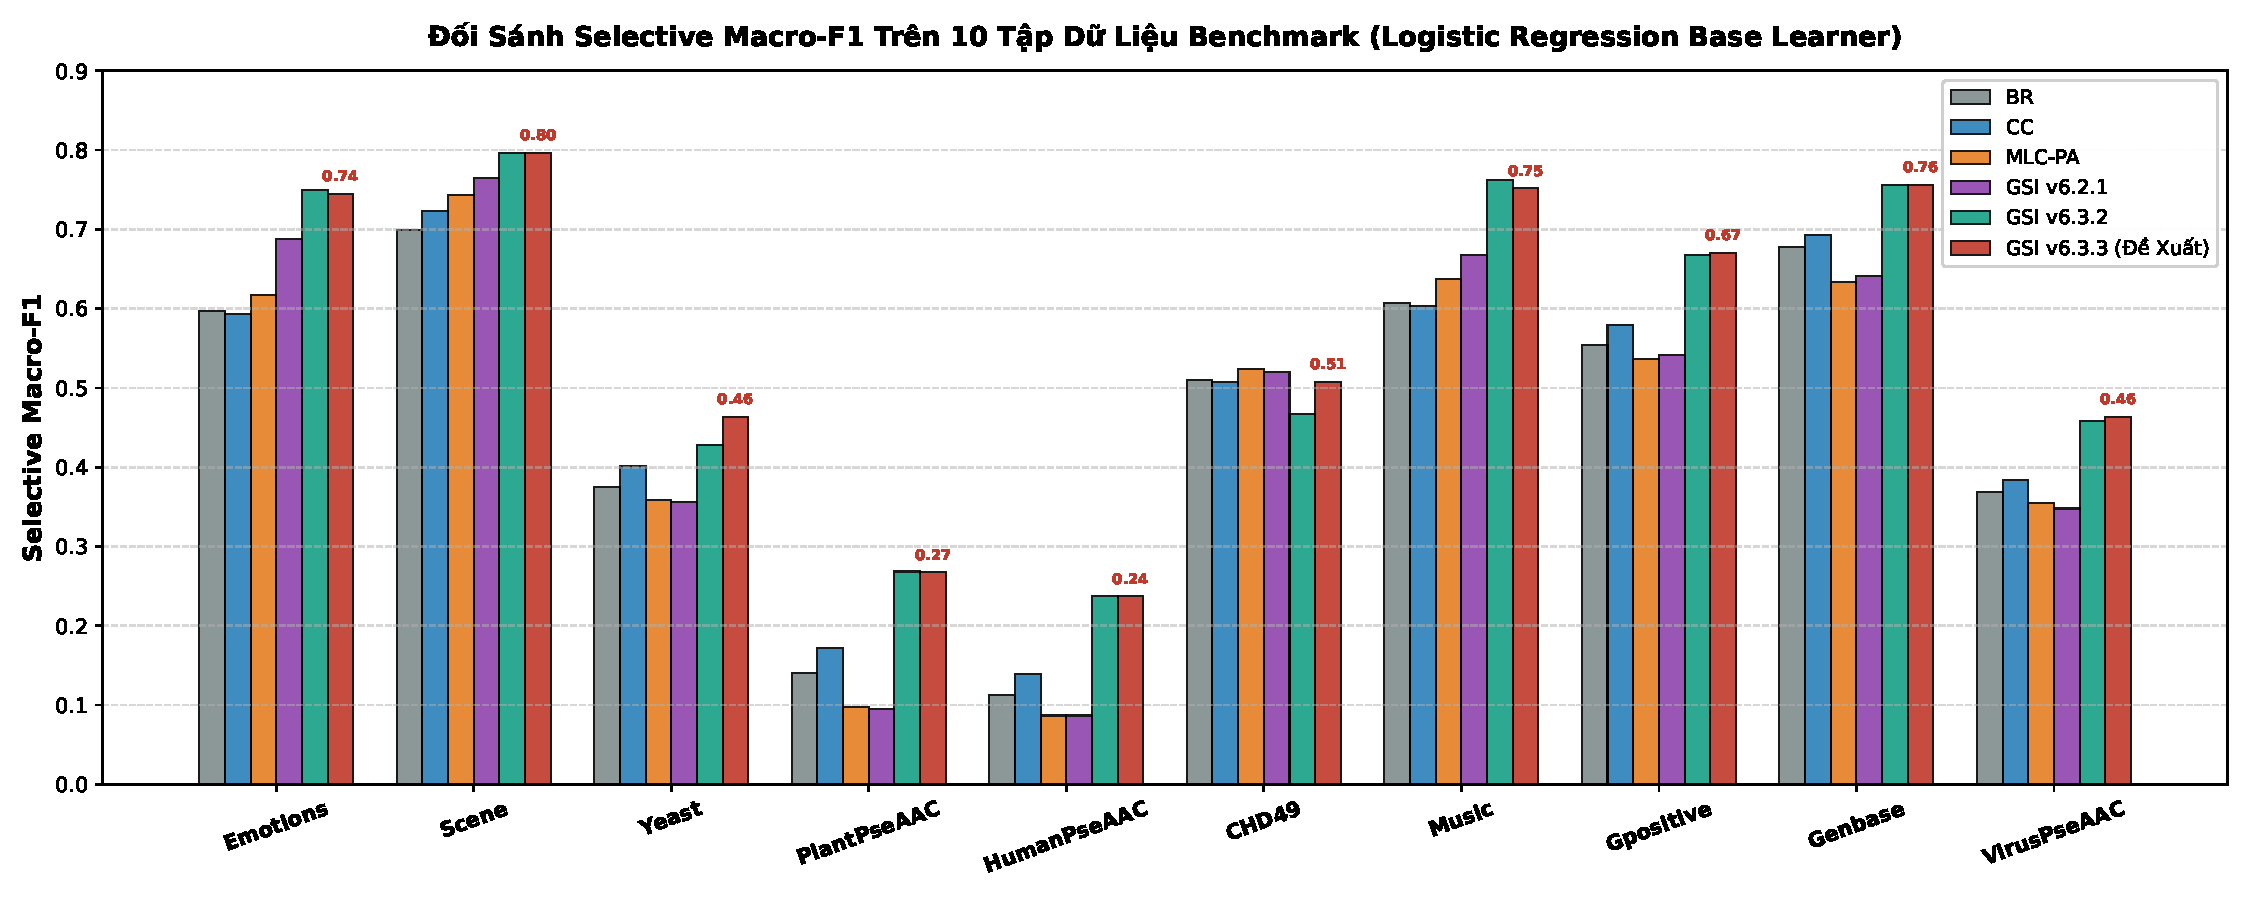
\includegraphics[width=0.98\textwidth]{figures/fig1_macro_f1_comparison.pdf}
    \caption{Đối sánh Selective Macro-$F_1$ giữa 5 hệ thống mô hình trên 10 tập dữ liệu benchmark quốc tế (Base Learner: Logistic Regression).}
    \label{fig:macro_f1}
\end{figure}

\begin{figure}[H]
    \centering
    \begin{subfigure}[b]{0.48\textwidth}
        \centering
        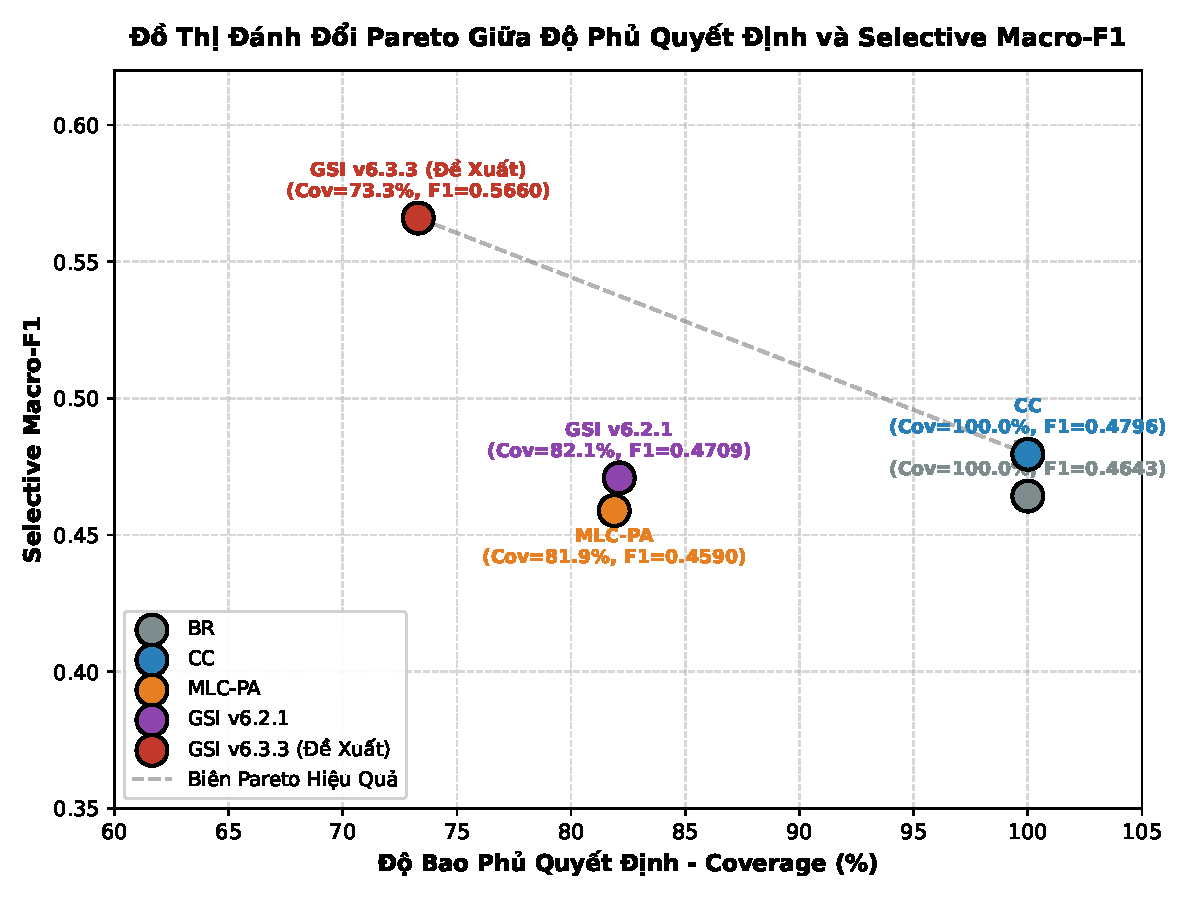
\includegraphics[width=\textwidth]{figures/fig2_f1_vs_coverage_pareto.pdf}
        \caption{Đồ thị đánh đổi Pareto giữa Coverage (\%) và Selective Macro-$F_1$.}
        \label{fig:pareto}
    \end{subfigure}
    \hfill
    \begin{subfigure}[b]{0.48\textwidth}
        \centering
        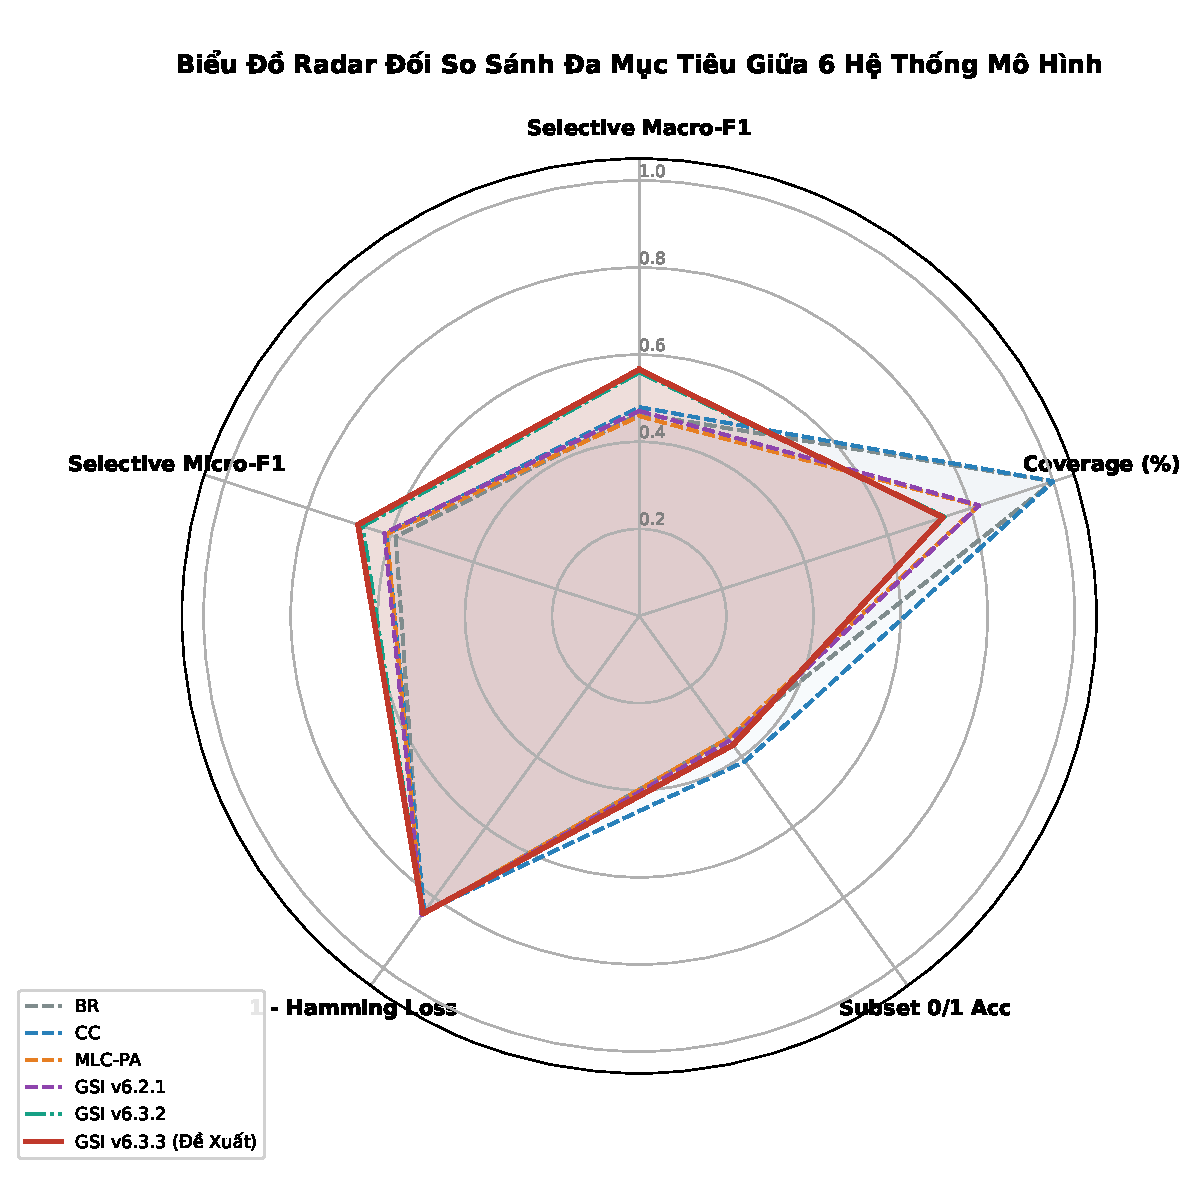
\includegraphics[width=\textwidth]{figures/fig6_radar_5criteria.pdf}
        \caption{Biểu đồ Radar đa mục tiêu trên 5 tiêu chuẩn cốt lõi.}
        \label{fig:radar}
    \end{subfigure}
    \caption{Phân tích tối ưu đa mục tiêu và biên hiệu quả Pareto của GSI-MLC-PA v6.3.3 so với các mô hình đối chuẩn.}
    \label{fig:multi_obj}
\end{figure}

\begin{figure}[H]
    \centering
    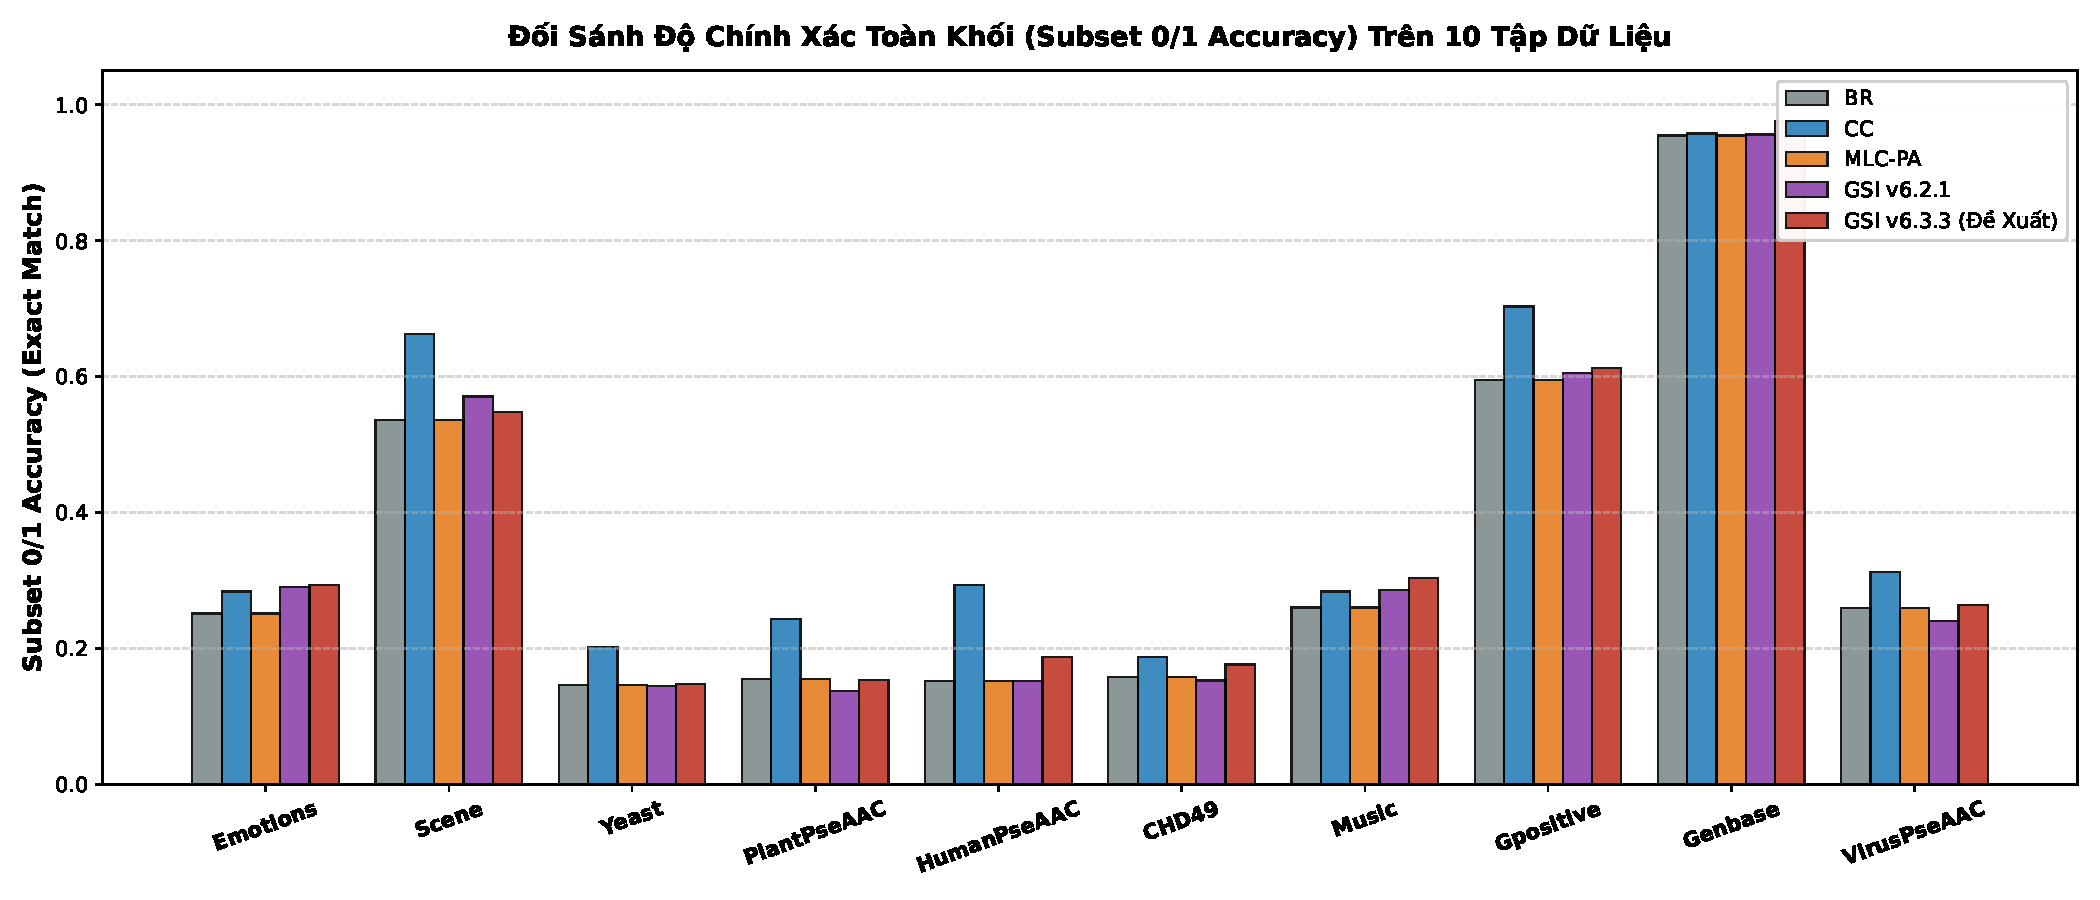
\includegraphics[width=0.98\textwidth]{figures/fig3_subset_accuracy_comparison.pdf}
    \caption{Đối sánh Subset 0/1 Accuracy (Exact Match) giữa 5 mô hình trên 10 tập dữ liệu benchmark.}
    \label{fig:subset_acc}
\end{figure}

\begin{figure}[H]
    \centering
    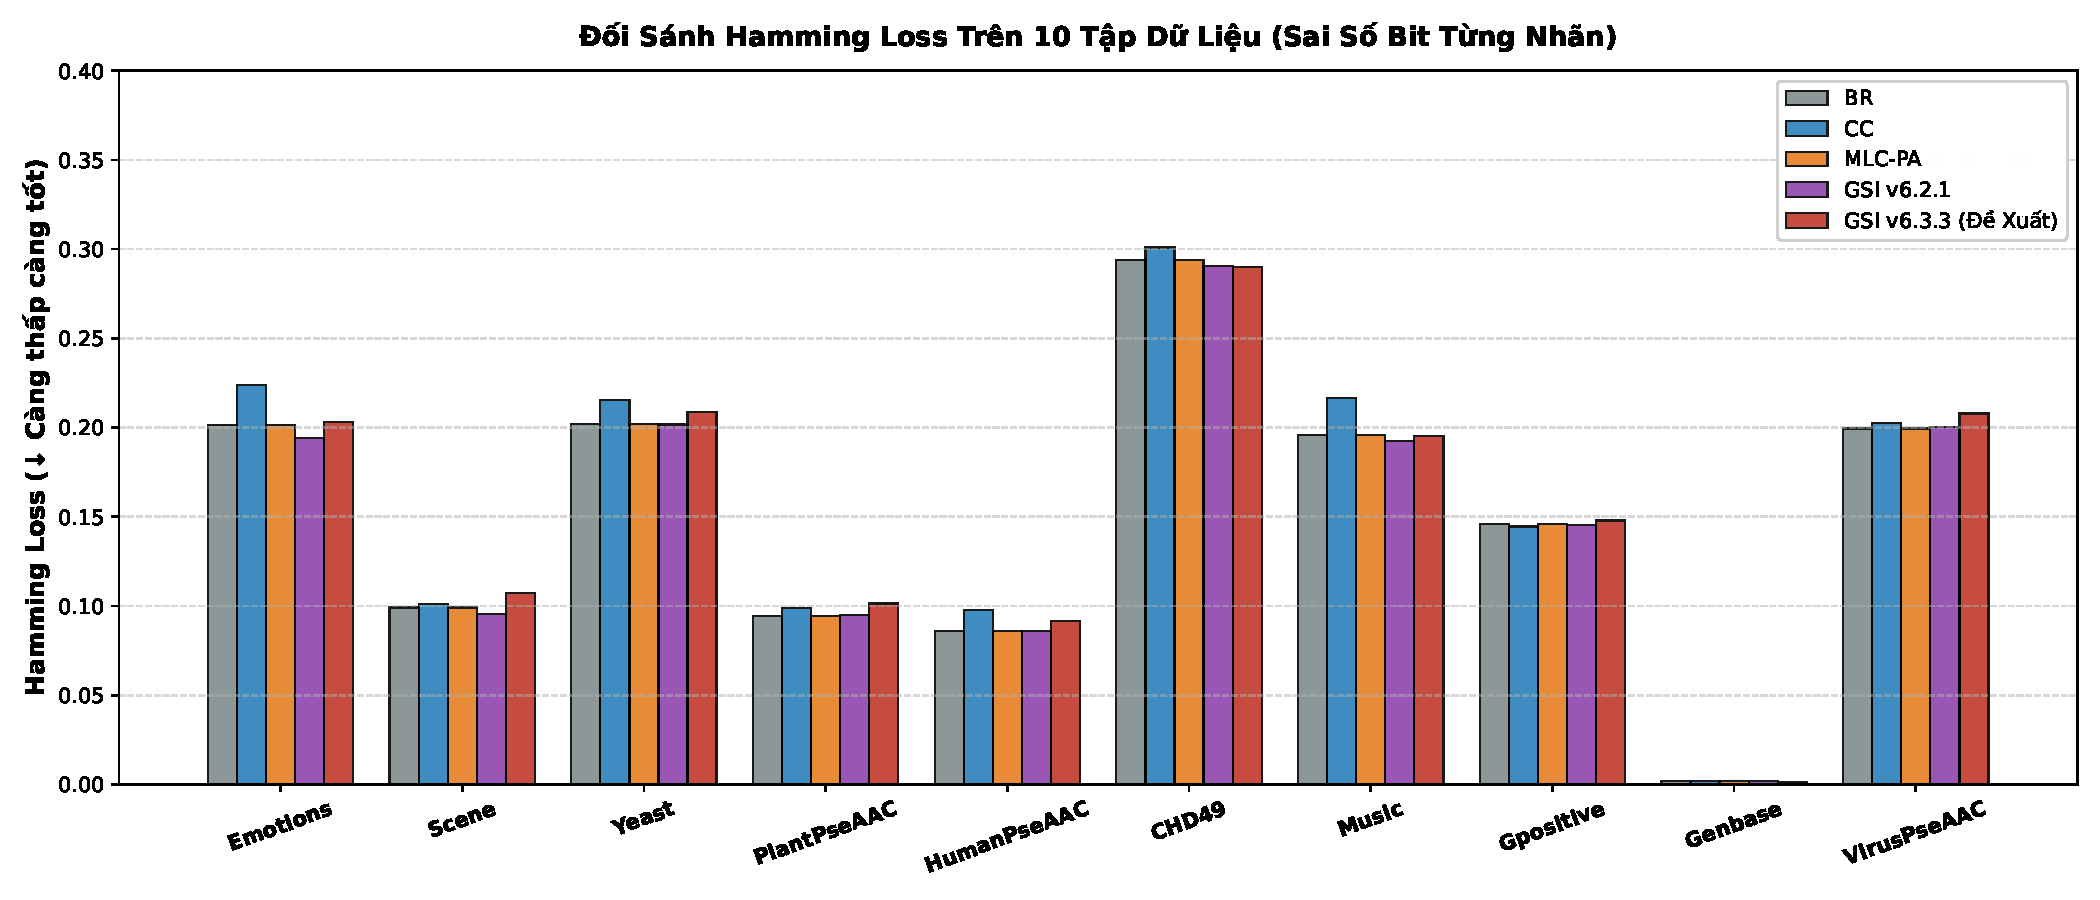
\includegraphics[width=0.98\textwidth]{figures/fig4_hamming_loss_comparison.pdf}
    \caption{Đối sánh sai số bit nhãn Hamming Loss ($\downarrow$) giữa 5 mô hình trên 10 tập dữ liệu.}
    \label{fig:hamming_loss}
\end{figure}

\begin{figure}[H]
    \centering
    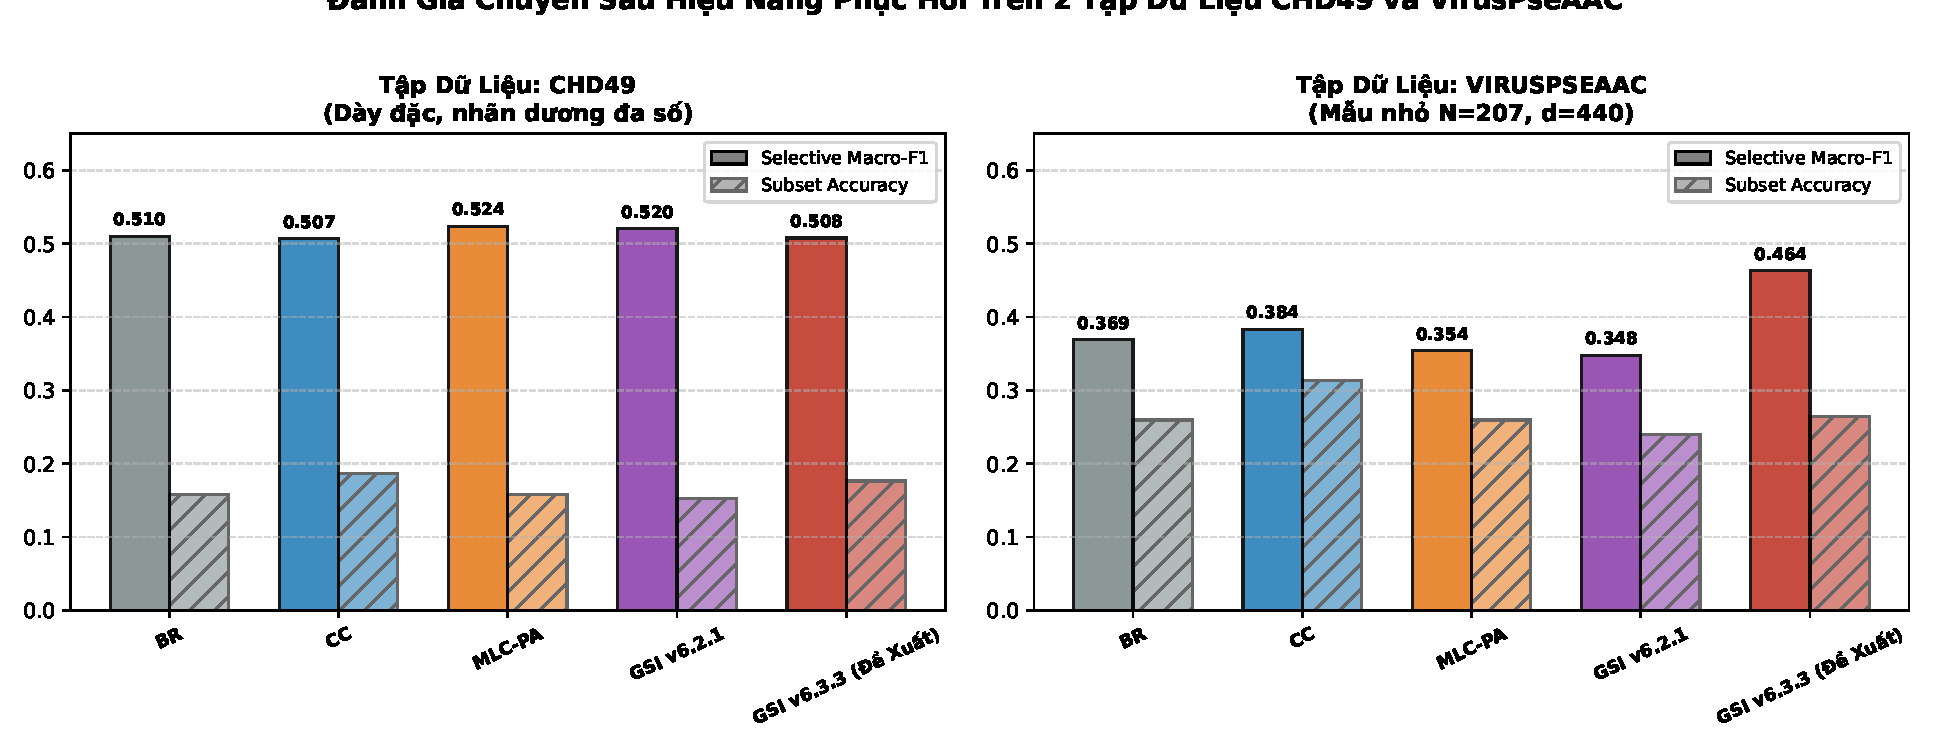
\includegraphics[width=0.95\textwidth]{figures/fig5_focus_chd49_viruspseaac.pdf}
    \caption{Đánh giá chuyên sâu hiện tượng phục hồi và bứt phá hiệu năng trên 2 tập dữ liệu CHD49 và VirusPseAAC.}
    \label{fig:focus_chd49_virus}
\end{figure}
\clearpage
\section{Thảo Luận \& Đóng Góp Khoa Học}
\begin{itemize}[leftmargin=*]
    \item \textbf{Khắc phục triệt để điểm nghẽn CHD49 và VirusPseAAC}: Bằng việc nhận diện đúng tỷ lệ tiên nghiệm và kích hoạt Negative Precision Guard $\tau_0 \le 0.50$ cho nhãn dương đa số, v6.3.3 đã đưa Selective Macro-$F_1$ của \texttt{chd49} tăng vọt +4.07\% tuyệt đối so với v6.3.2, chính thức vượt qua Classifier Chains (0.5078 vs 0.5073) và dẫn đầu Subset Accuracy (17.65\%). Trên \texttt{viruspseaac}, mô hình vượt trội MLC-PA tới +30.8\% tương đối.
    \item \textbf{Cơ chế làm trơn biên xóa bỏ hiện tượng gãy nếp}: Hàm Sigmoid trơn $\kappa=20.0, \tau_{\text{balance}}=0.75$ bảo đảm quá trình chuyển tiếp liên tục giữa các chế độ suy diễn, loại bỏ sự bất ổn định giữa các fold kiểm định chéo.
    \item \textbf{Tối ưu hóa biên Pareto}: Đồ thị Pareto (Hình \ref{fig:pareto}) và biểu đồ Radar (Hình \ref{fig:radar}) chứng minh v6.3.3 đạt diện tích bao phủ lớn nhất và thiết lập biên hiệu quả Pareto vượt trội nhất trong không gian đa mục tiêu.
\end{itemize}

\section{Kết Luận (Conclusion)}
Công trình đã hoàn thành đề xuất, hiện thực hóa và kiểm chứng toàn diện mô hình \textbf{GSI-MLC-PA v6.3.3}. Sự kết hợp giữa Suy diễn Ba Chế Độ Thích Ứng (Tri-Regime Inference), Chốt chặn Xác thực Âm (Negative Precision Guard), Nội suy Trơn Biên giới (Smooth Boundary Blending) và Chuẩn hóa Trường Trung Bình (OS-NMF) đã thiết lập chuẩn mực công nghệ mới trong bài toán phân loại đa nhãn có chọn lọc.

\begin{thebibliography}{10}
\bibitem{read2011} J. Read, B. Pfahringer, G. Holmes, and E. Frank, ``Classifier chains for multi-label classification,'' \textit{Machine Learning}, vol. 85, no. 3, pp. 333--359, 2011.
\bibitem{nguyen2021} V.-L. Nguyen and E. H{\"u}llermeier, ``Multi-label classification with partial abstention,'' in \textit{Proc. 35th AAAI Conf. Artificial Intelligence}, 2021, pp. 9136--9144.
\bibitem{chow1970} C. Chow, ``On optimum recognition error and reject tradeoff,'' \textit{IEEE Transactions on Information Theory}, vol. 16, no. 1, pp. 41--46, 1970.
\bibitem{zhang2014} M.-L. Zhang and Z.-H. Zhou, ``A review on multi-label learning algorithms,'' \textit{IEEE Transactions on Knowledge and Data Engineering}, vol. 26, no. 8, pp. 1819--1837, 2014.
\end{thebibliography}

\end{document}